% id: 150-298
% book: 개념원리 기하 · 19 벡터의 덧셈과 뺄셈
% section: 개념원리 익히기
% figure: crop:fig-150-298.png
% answer: 풀이 참조 (모눈 한 칸을 단위로 ⑴ 왼쪽 $1$, 위 $2$ ⑵ 오른쪽 $3$, 아래 $1$ ⑶ 왼쪽 $6$, 아래 $6$인 화살표 $\vec{a}-\vec{b}$를 그린 그림 — 답지 참조)
% answer_source: 답지(그림)
% variant_level: 0 (원본 전사)
% 이 파일은 build.mjs 가 items.json 에서 만든다. 고칠 때는 items.json 을 고친다.
\smash{\raisebox{1.5mm}{\dmkichul{개념원리 기하 150쪽 298번}}}
두 벡터 $\vec{a}$, $\vec{b}$가 다음 그림과 같을 때, $\vec{a}-\vec{b}$를 그림으로 나타내시오.
\par\smallskip\begin{center}\setlength{\dmfigw}{272.5pt}\ifdim\dmfigw>\linewidth\setlength{\dmfigw}{\linewidth}\fi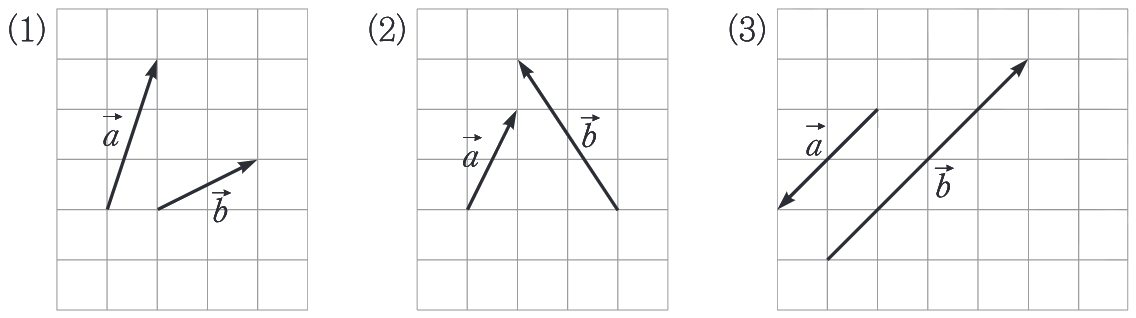
\includegraphics[width=\dmfigw]{figures/fig-150-298.png}\end{center}
